\newpage

\section{Appendix - Alternatives}
\label{sec:dp-pds-appendix}

\subsection{Individual Ground Grids}
\label{sec:dp-pds-appendix-grid}

In collaboration with the \dword{hv} consortium, the installation of individual \dwords{gg} for each \dword{pmt} in place of the \dword{gg} table structure is under consideration. Since the individual \dword{gg} cages will potentially have thinner wires and be closer to the \dword{pmt} windows, thereby generating a smaller shadow, they should increase the acceptance of the \dwords{pmt}.

The feasibility of the design in operation under \dword{dpmod} conditions will be studied by the \dword{hv} consortium. The design of the individual grids will be developed as a common effort of the two consortia engineering teams. The \dword{hv} consortium will produce the grids. The grids will be installed at the \dword{ctsf} by \dword{dp} \dword{pds} consortium. This same consortium will install the  \dwords{pmt} %will be installed 
with their individual grid cages. 

\subsection{Calibration System Alternatives}
\label{sec:dp-pds-appendix-calibration}

Alternatives to the baseline design of the calibration system described in Section~\ref{sec:dp-pds-calibration} will be pursued with R\&D measurements in order to make the system more effective, reduce the cost, and mitigate issues related to scaling to the \dword{dpmod} size. These alternatives include reducing the number of fibers, studying other options for the reference sensor, and increasing the input light, if necessary. To reduce the number of fibers, light diffusers can be used, so that one fiber can illuminate at least four \dwords{pmt}. For instance, a diffuser could be placed at the \dword{gg}, or in the case of individual \dwords{gg}, on the side walls. With the same aim of reducing the total number of fibers, an alternative calibration system with two fibers placed at the top of the \dword{fc} is being tested in \dword{pddp}, so that one fiber can illuminate several \dwords{pmt}. Other %than the diffusers and fiber placement, 
considered alternatives relate to the external system and can be implemented with minimal interference with other subsystems.

\subsection{Xenon Doping of Liquid Argon}
\label{sec:dp-pds-appendix-xedoping}

Doping the \dword{lar} volume with xenon is an attractive option in terms of providing %a 
volume-distributed wavelength shifting. Major advantages of xenon doping are enabling the long-lived triplet Ar excimer to produce a faster signal, reducing the fraction of late light, and shifting the scintillation signal to longer wavelengths (\SI{175}{nm}). As a consequence of the latter, the Rayleigh scattering length will be longer.

Dedicated simulations on light yield in the full \dword{dpmod} cryostat in the presence of xenon doping were performed. Figure~\ref{fig:dppd_fd_light_yield_xedoping} shows the 1D light yields as a function of the drift (transverse) direction in the left (right) panel, averaging over the other two spatial coordinates. It is evident that the xenon doping can be considered as an immediate alternative to the baseline design with half-coverage reflector/\dword{wls} panels in terms of light output. On the other hand, keeping a smaller area coverage reflector/\dword{wls} panels closer to the charge readout may be preferable in order to improve the uniformity. 
\fixme{I think this sentence means: On the other hand, instead of doping with xenon, it may improve the uniformity to keep the half-coverage reflector/\dword{wls} panels closer to the charge readout.}


\begin{dunefigure}[Expected 1D light yields in the full \dshort{dpmod} with xenon doping]{fig:dppd_fd_light_yield_xedoping}
{Expected light yield in the full \dword{dp} \dword{fd} cryostat in the presence of xenon doping. The yield units are number of \phel{}s per \si{\MeV} of deposited energy. The 1D yields are shown as a function of the drift (transverse) direction in the left (right) panel, averaging over the other two spatial coordinates (not shown), similarly to Figure~\ref{fig:dppd_fd_light_yield_comparisons}. The three histograms correspond to the half-foil baseline design without xenon doping, and to two no-foil geometries, with and without xenon doping, respectively.}
\raisebox{0.1cm}{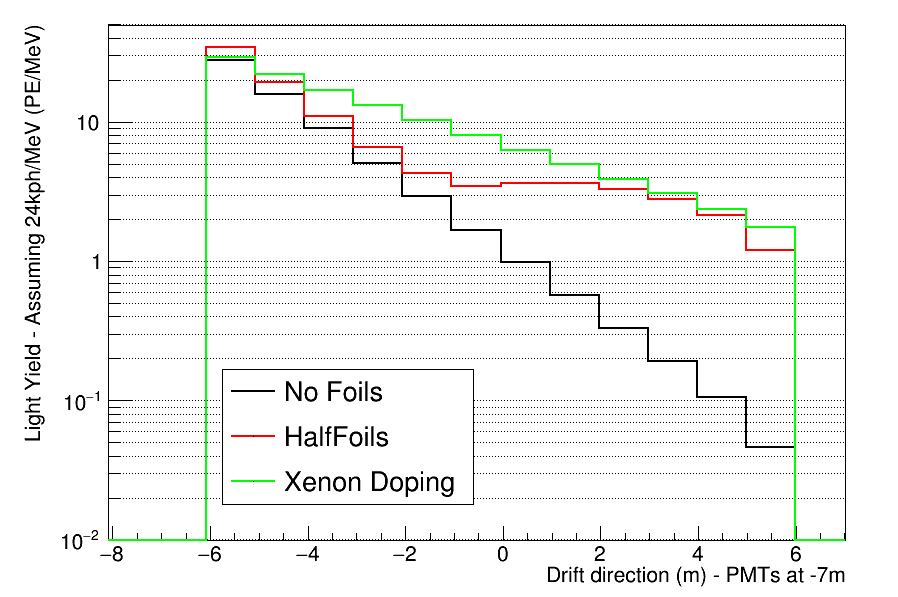
\includegraphics[width=0.49\textwidth]{graphics/dppd_xedoping_drift.png}} \hfill
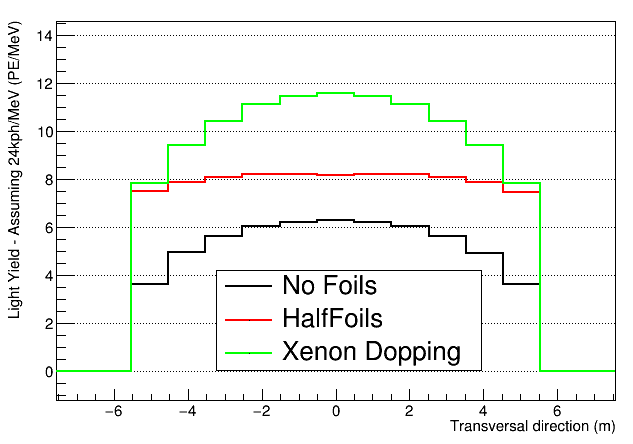
\includegraphics[width=0.49\textwidth]{graphics/dppd_xedoping_transverse.png}
\end{dunefigure}